\chapter{复变函数}

	\section{复数与复变函数}
	在本章中,首先结束复数系统的代数和几何结构。然后引进复变量的函数——复变函数,进而介绍他的连续性和连续性。
	
	\subsection{复数和四则运算}
	
	\subsubsection{复数的基本概念}
	为了便于后文说明,这里简单介绍复数的基本定义和结论。
	\begin{definition}{复数}{Complex number}
	设$x$和$y$为两实数,称形如
	\begin{equation}
	z =  x+\mathrm{i} y ~ (\mbox{或} x+y\mathrm{i})
	\end{equation}
	的数称为\hint{复数}。这里$\mathrm{i}$为虚数单位,具有性质$\mathrm{i}^2 = 1$,$x$和$y$分别称为复数$z$的实部和虚部。复数集记为$\mathbb{C}$,常记做
	$$ x = \mathrm{Re}\left(z\right),\quad y =  \mathrm{Im}\left(z\right).$$		
	\end{definition}
	虚部为零的数称为实数,简记为$x + \mathrm{i} 0 = x$,实数集记为$\mathbb{R}$。因此,全体实数为复数的一部分,特别的有
	$0 + \mathrm{i} 0 = 0$,即当且实部和虚部同时为零时$z$为零。当虚部不为零的复数称为\hint{虚数},而实部为零且虚部不为零的复数称为\hint{纯虚数}。如果量两复数的实部和虚部分别相等,则称两复数\hint{相等}。
	
	\subsubsection{复数的四则运算}
	\begin{theorem}{复数的四则运算}
		设$z_1$和$z_2$为两个复数
		$$z_1 =  x_1+\mathrm{i} y_1,\quad z_2 =  x_2+\mathrm{i} y_2.$$
		定义两复数$z_1$,$z_2$的四则运算为
		\begin{subequations}
			\renewcommand{\theequation}{\theparentequation-\arabic{equation}}
			\begin{align}  
			{}&z_1+z_2 = \left(x_1+\mathrm{i} y_1\right) +\left(x_2+\mathrm{i} y_2\right) = \left(x_1+x_2\right)+\mathrm{i}\left(y_1+y_2\right)                                   \label{eq:complex41} \\
			{}&z_1-z_2 = \left(x_1+\mathrm{i} y_1\right) -\left(x_2+\mathrm{i} y_2\right) = \left(x_1-x_2\right)+\mathrm{i}\left(y_1-y_2\right)                                  \label{eq:complex42} \\
			{}&z_1 \cdot z_2 = \left(x_1+\mathrm{i} y_1\right) \cdot \left(x_2+\mathrm{i} y_2\right) = \left(x_1x_2-y_1y_2\right)+\mathrm{i}\left(x_1y_2+y_1x_2\right)                                            \label{eq:complex43}
			\end{align}
			若$z_2 \ne 0$,则
			\begin{equation}
				\frac{z_1}{z_2} = \frac{x_1+\mathrm{i} y_1}{x_2+\mathrm{i} y_2} = \frac{\left(x_1+\mathrm{i} y_1\right)\left(x_2-\mathrm{i} y_2\right)}{\left(x_2+\mathrm{i} y_2\right)\left(x_2-\mathrm{i} y_2\right)} = \frac{x_1x_2+y_1y_2}{x^2_2+y^2_2} +\mathrm{i}\frac{x_2y_1-x_1y_2}{x^2_2+y^2_2}  \label{eq:complex44}
			\end{equation}
		\end{subequations}	
	\end{theorem}
	从式~\ref{eq:complex41}$\sim$式~\ref{eq:complex44} 可知复数经过四则运算仍然是复数,又从式~\ref{eq:complex41} 和式~\ref{eq:complex42} 以及虚部和实部的定义可知
	\begin{subequations}
		\renewcommand{\theequation}{\theparentequation-\arabic{equation}}
		\begin{align}  
			{}& \mathrm{Re}\left(z_1 \pm z_2\right) = \mathrm{Re}\left(z_1\right) \pm \mathrm{Re}\left(z_2\right) \label{eq:complex51} \\
			{}& \mathrm{Im}\left(z_1 \pm z_2\right) = \mathrm{Im}\left(z_1\right) \pm \mathrm{Re}\left(z_2\right) \label{eq:complex52} 
		\end{align}
	\end{subequations}

	\begin{example}
		\begin{enumerate}[noitemsep]
		\item 
		化简 $\displaystyle i^3,\frac{\mathrm{i}}{1-\mathrm{i}}+\frac{1-\mathrm{i}}{\mathrm{i}}. $
		\item 计算 (1)  $\displaystyle \frac{2+3\mathrm{i}}{2-3\mathrm{i}}$,\quad (2)  $\displaystyle \frac{2\mathrm{i}}{\sqrt{3}-\mathrm{i}}-\frac{3}{\sqrt{3}\mathrm{i}-1}$。
		\item 已知$x+y\mathrm{i} = \left(2x-1\right)+y^2\mathrm{i}$,求$z = x+\mathrm{i}y$。 
		\end{enumerate}
	\end{example}
	
	\begin{solution} 
		\begin{enumerate}[noitemsep]
			\item $\displaystyle -\mathrm{i},\quad -\frac{3}{2}-\frac{1}{2}\mathrm{i}$。
			\item (1) $\displaystyle -\frac{5}{13}+\frac{12}{13}\mathrm{i}$, \quad (2) $\displaystyle \frac{1}{4}+\frac{5\sqrt{3}}{4}\mathrm{i}$。
			\item $z = 1$ 或 $z = 1+\mathrm{i}$。
		\end{enumerate}
	\end{solution}

	\subsection{复数的几何表示}
	\subsubsection{复数的向量表示和复平面}
	任意给定的一个复数$z =  x+\mathrm{i}$,都有一对有序实数$\left(x,y\right)$相对应,而任意一对有序实数$\left(x,y\right)$都与直角坐标系$P\left(x,y\right)$对应。只有能够建立盘面上的全部点与全体复数简的一一对应关系,于是可用直角坐标系中的点来表示复数,如\figref{fig:vectorcomple}所示。
	
	\usetikzlibrary{angles}
	\usetikzlibrary{quotes}
	\begin{figure}[ht]
		\centering
		\begin{tikzpicture}[scale = 2]
		% \draw[step=1] (-0.5,-0.2) grid (4,3);
		\draw[-stealth,line width = 0.8pt] (-1.5,0) -- (4,0)node[below,scale=1]{$x$};
		\draw[-stealth,line width = 0.8pt] (0,-0.3) -- (0,3)node[right,scale=1]{$y$};
		\draw[-stealth,line width = 1pt,color = blue](0,0) -- (3,2.2);
		\draw[dashed,line width = 0.8pt,color = red](3,0) -- (3,2.2);
		\draw[dashed,line width = 0.8pt,color = red](0,2.2) -- (3,2.2);
		\node[below left] (n1) at (0.05, 0.05){$O$};
		\node[above right] (n2) at (2.95, 1.85){$P(x,y)$};
		\node[above right] (n3) at (2.75, 2.15){$z = x+ \mathrm{i}y$};
		\node[above left] (n4) at (1.5, 1){$r$};	
		\draw(2,0) coordinate (A) (0,0) coordinate (B) (3,2.2) coordinate (C) pic[draw,"$\theta$ ",line width = 1pt,angle eccentricity =1.2,-stealth,angle radius = 1cm]{angle};
		\end{tikzpicture}
		\caption{向量的几何表示}
		\label{fig:vectorcomple}
	\end{figure}
	
	表示复数$z$的直角坐标平面称为\hint{复平面}或 \hint{$z-$平面},复平面也常用集合$\mathbb{C}$来表示。因复平面上的$x$轴上的点对应实数,$y$轴上非零的点对应纯虚数,因此称$x$轴为实轴,$y$轴为虚轴。由于全体复数与复平面上的点的全体是一一对应的,以后吧“点$z$”和“复数$z$”作为同义词而不加以区别。
	
	在复平面上,如\figref{fig:vectorcomple}所示,从原点$O$到点$P\left(x,y\right)$作向量$\overrightarrow{OP}$。我们可以看到复平面上由原点$O$出发的向量的 全体和复数的全体$\mathbb{C}$之间也构成一一对应关系(复数$0$对应着零向量),因此也可以向量$\overrightarrow{OP}$来表示复数$z =  x+\mathrm{i}y$,其中$x$,$y$分别等于向量$\overrightarrow{OP}$沿$x$轴与$y$轴的分量。今后把“复数$z$”与其对应的向量$z$”也视为同义词。
	
	在物理学中,如力、速度、加速度等都可用向量表示,说明复数可以用来表示实有的物理量。
	
	\subsubsection{模与辐角}
	\begin{definition}{模与辐角}{abs and angle}
		向量$\overrightarrow{OP}$的长度$r$叫做复数$z$的\hint{模}或\hint{绝对值},记作$|z|$,即$|z| = r$。实轴正向转到与向量$\overrightarrow{OP}$方向一致时所成的角度叫做复数的\hint{辐角},记作$\mathrm{Arg} \left(z\right)$,即$\mathrm{Arg}\left(z\right)=\theta$。	
	\end{definition}
	
	复数$0$的模为零,即$|0|=0$,其辐角是不确定的。任何不为零的复数$z$的辐角$\mathrm{Arg} \left(z\right)$均有无穷多个值彼此之间相$2\pi$的整数倍通常把满足$-\pi < \theta \ne \pi$的辐角值$\theta_0$称为$\mathrm{Arg} \left(z\right)$的主值记为$\mathrm{arg} \left(z\right)$,于是
	\begin{equation}
	\mathrm{Arg} \left(z\right)=\mathrm{arg} \left(z\right)+ 2k\pi,\quad ,k=0,\pm1,\pm2,\cdots
	\end{equation}
	并且可以用复数$z$的实部来表示辅角的主值$\mathrm{arg} \left(z\right)$:
	\begin{equation}
	\arg z = \begin{dcases}
	  {\arctan \frac{y}{x},} & {x>0} \\
	  {\arctan \frac{y}{x}+\pi,} & {x>0, y>0} \\ 
	  {\arctan \frac{y}{x}-\pi,} & {x<0, y>0}\\
	  \end{dcases}
	\end{equation}
	
	由直角坐标与极坐标的关系(\figref{fig:vectorcomple}),我们立即得到不为零的复数的实部、虚部与该复数的模、辐角之间的关系
	\begin{equation}
	\left\{ 
	\begin{aligned}
	{}&r = |z| = \sqrt{x^2+y^2}\\
	{}&\tan\left(\theta\right) = \tan\left(	\mathrm{Arg} \left(z\right)\right) = \frac{y}{x}\\
	\end{aligned}
	\right. 
	\end{equation}
	
	以及
	\begin{equation}
	\left\{ 
	\begin{aligned}
	{}& x = z\cos \\
	{}&\tan\left(\theta\right) = \tan\left(	\mathrm{Arg} \left(z\right)\right) = \frac{y}{x}\\
	\end{aligned}
	\right. 
	\end{equation}
	
	于是复数z又可表示为
	
	a =r t	(cos0- ising	
	
	(1.2.3)式通常称为复数z的三角表示式如果再利用欧拉( Euler)公式
	
	
	我们又可以得到
	
	
	这种形式称为复数的指数表示式
	
	在§11节中已经指出:两复数的实部与虚部分别相等则称两复数相等.于
	
	是从(12.1)式与(122)式即知两复数相等,其模必定相等其辐角可以差2x的
	
	
	\begin{figure}[ht]
		\centering
		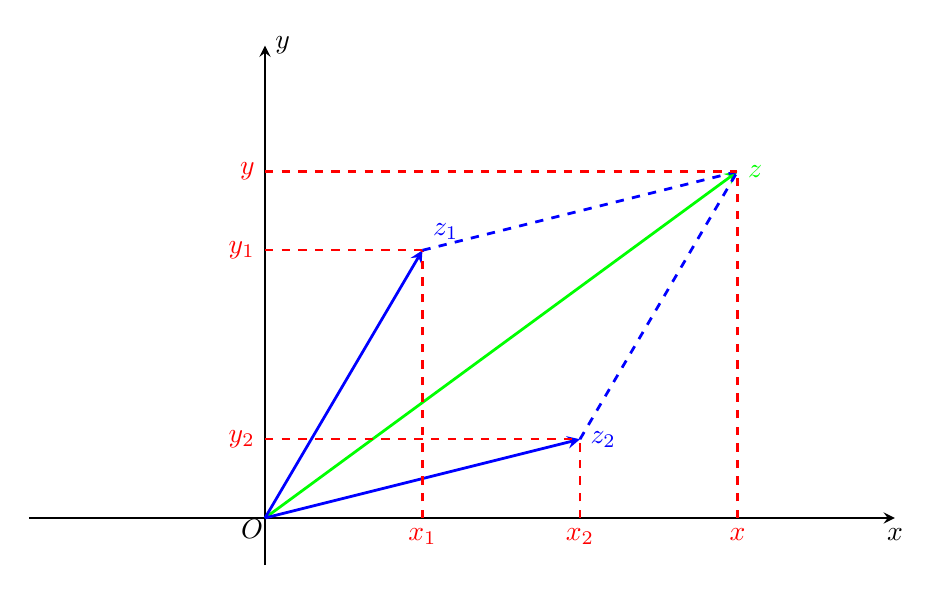
\begin{tikzpicture}[scale = 2]
		\draw[-stealth,line width = 0.8pt] (-1.5,0) -- (4,0)node[below,scale=1]{$x$};
		\draw[-stealth,line width = 0.8pt] (0,-0.3) -- (0,3)node[right,scale=1]{$y$};
		\draw[-stealth,line width = 1pt,color = green](0,0) -- (3,2.2)node[right,scale=1]{$z$};
		\draw[-stealth,line width = 1pt,color = blue](0,0) -- (2,0.5)node[right,scale=1]{$z_2$};
		\draw[dashed,line width = 0.8pt,color = red](2,0)node[below,scale=1]{$x_2$} -- (2,0.5);
		\draw[dashed,line width = 0.8pt,color = red](0,0.5)node[left,scale=1]{$y_2$}-- (2,0.5);
		\draw[-stealth,line width = 1pt,color = blue](0,0) -- (1,1.7)node[above right,scale=1]{$z_1$};
		\draw[dashed,line width = 0.8pt,color = red](0,1.7)node[left,scale=1]{$y_1$} -- (1,1.7);
		\draw[dashed,line width = 0.8pt,color = red](1,0)node[below,scale=1]{$x_1$}  -- (1,1.7);
		\draw[dashed,line width = 1pt,color = blue](2,0.5) -- (3,2.2);
		\draw[dashed,line width = 1pt,color = blue](1,1.7) -- (3,2.2);
		\draw[dashed,line width = 0.8pt,color = red](3,0)node[below,scale=1]{$x$} -- (3,2.2);
		\draw[dashed,line width = 0.8pt,color = red](0,2.2)node[left,scale=1]{$y$} -- (3,2.2);
		\node[below left] (n1) at (0.05, 0.05){$O$};
		\end{tikzpicture}
		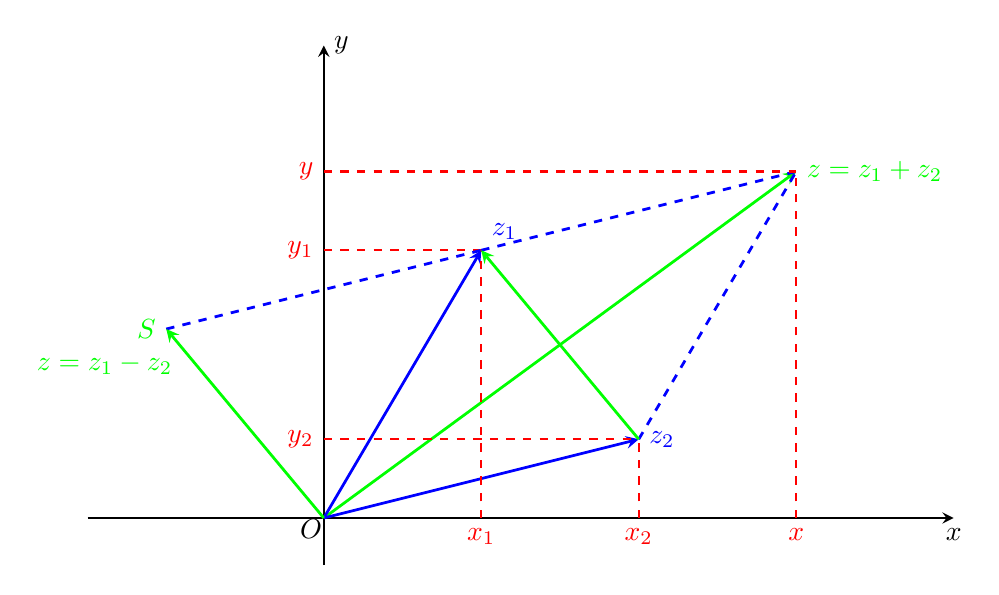
\begin{tikzpicture}[scale = 2]
		\draw[-stealth,line width = 0.8pt] (-1.5,0) -- (4,0)node[below,scale=1]{$x$};
		\draw[-stealth,line width = 0.8pt] (0,-0.3) -- (0,3)node[right,scale=1]{$y$};
		\draw[-stealth,line width = 1pt,color = green](0,0) -- (3,2.2)node[right,scale=1]{$z = z_1+z_2$};
		\draw[-stealth,line width = 1pt,color = blue](0,0) -- (2,0.5)node[right,scale=1]{$z_2$};
		\draw[dashed,line width = 0.8pt,color = red](2,0)node[below,scale=1]{$x_2$} -- (2,0.5);
		\draw[dashed,line width = 0.8pt,color = red](0,0.5)node[left,scale=1]{$y_2$}-- (2,0.5);
		\draw[-stealth,line width = 1pt,color = blue](0,0) -- (1,1.7)node[above right,scale=1]{$z_1$};
		\draw[dashed,line width = 0.8pt,color = red](0,1.7)node[left,scale=1]{$y_1$} -- (1,1.7);
		\draw[dashed,line width = 0.8pt,color = red](1,0)node[below,scale=1]{$x_1$}  -- (1,1.7);
		\draw[dashed,line width = 1pt,color = blue](2,0.5) -- (3,2.2);
		\draw[dashed,line width = 1pt,color = blue](1,1.7) -- (3,2.2);
		\draw[dashed,line width = 0.8pt,color = red](3,0)node[below,scale=1]{$x$} -- (3,2.2);
		\draw[dashed,line width = 0.8pt,color = red](0,2.2)node[left,scale=1]{$y$} -- (3,2.2);
		\node[below left] (n1) at (0.05, 0.05){$O$};
		\draw[-stealth,line width = 1pt,color = green](2,0.5) -- (1,1.7);
		\draw[dashed,line width = 1pt,color = blue](-1,1.2) -- (1,1.7);
		\draw[-stealth,line width = 1pt,color = green](0,0) -- (-1,1.2)node[left,scale=1]{$S$};
		\node[below left,color = green] (n1) at (-0.9,1.1){$z = z_1-z_2$};
		\end{tikzpicture}
		\caption{复数的加减法}
		\label{fig:complemp}
	\end{figure}

	\subsection{共轭复数}
	
	\subsection{复数的乘除、乘方和开方}
	
	\subsection{复球面与无穷远点}